% !TEX encoding = UTF-8 Unicode
\documentclass[a4paper]{article}

\usepackage{color}
\usepackage{url}
\usepackage[T2A]{fontenc} % enable Cyrillic fonts
\usepackage[utf8]{inputenc} % make weird characters work
\usepackage{graphicx}

\usepackage[english,serbian]{babel}
%\usepackage[english,serbianc]{babel} %ukljuciti babel sa ovim opcijama, umesto gornjim, ukoliko se koristi cirilica

\usepackage{float}
\usepackage[unicode]{hyperref}
\hypersetup{colorlinks,citecolor=green,filecolor=green,linkcolor=blue,urlcolor=blue}

\usepackage{listings}

%\newtheorem{primer}{Пример}[section] %ćirilični primer
\newtheorem{primer}{Primer}[section]

\definecolor{mygreen}{rgb}{0,0.6,0}
\definecolor{mygray}{rgb}{0.5,0.5,0.5}
\definecolor{mymauve}{rgb}{0.58,0,0.82}

\lstset{ 
  backgroundcolor=\color{white},   % choose the background color; you must add \usepackage{color} or \usepackage{xcolor}; should come as last argument
  basicstyle=\scriptsize\ttfamily,        % the size of the fonts that are used for the code
  breakatwhitespace=false,         % sets if automatic breaks should only happen at whitespace
  breaklines=true,                 % sets automatic line breaking
  captionpos=b,                    % sets the caption-position to bottom
  commentstyle=\color{mygreen},    % comment style
  deletekeywords={...},            % if you want to delete keywords from the given language
  escapeinside={\%*}{*)},          % if you want to add LaTeX within your code
  extendedchars=true,              % lets you use non-ASCII characters; for 8-bits encodings only, does not work with UTF-8
  firstnumber=1000,                % start line enumeration with line 1000
  frame=single,	                   % adds a frame around the code
  keepspaces=true,                 % keeps spaces in text, useful for keeping indentation of code (possibly needs columns=flexible)
  keywordstyle=\color{blue},       % keyword style
  language=Python,                 % the language of the code
  morekeywords={*,...},            % if you want to add more keywords to the set
  numbers=left,                    % where to put the line-numbers; possible values are (none, left, right)
  numbersep=5pt,                   % how far the line-numbers are from the code
  numberstyle=\tiny\color{mygray}, % the style that is used for the line-numbers
  rulecolor=\color{black},         % if not set, the frame-color may be changed on line-breaks within not-black text (e.g. comments (green here))
  showspaces=false,                % show spaces everywhere adding particular underscores; it overrides 'showstringspaces'
  showstringspaces=false,          % underline spaces within strings only
  showtabs=false,                  % show tabs within strings adding particular underscores
  stepnumber=2,                    % the step between two line-numbers. If it's 1, each line will be numbered
  stringstyle=\color{mymauve},     % string literal style
  tabsize=2,	                   % sets default tabsize to 2 spaces
  title=\lstname                   % show the filename of files included with \lstinputlisting; also try caption instead of title
}

\begin{document}

\title{Idealne studije\\ \small{Seminarski rad u okviru kursa\\Metodologija stručnog i naučnog rada\\ Matematički fakultet}}

\author{Bojan Veličković 1070/2024, David Živković 1027/2024\\ Darko Mladenovski 1067/2024, Marko Radosavljević 1010/2024\\bojanvelickovic76@gmail.com, dzivkovicd1@gmail.com,\\ darkomladenovski0@gmail.com, 01marko.radosavljevic@gmail.com}


%\date{9.~april 2015.}

\maketitle

\abstract{
Cilj ovog rada je da ispita kako studenti ocenjuju važnost kriterijuma, postavljenih od strane autora, koji treba da važe kako bi studije bile idealne. Pored toga, proverava se i koliko su ti kriterijumi, na osnovu iskustva studenata, prisutni na Matematičkom fakultetu. Rezultati pokazuju da je zadovoljstvo studenata kursevima, njihova organizacija kao i koliko spremaju studente za svoje karijere nakon studija veoma važni. Pored toga toga ističe se i doprinos organizacije na fakultetu kako bi studije bile idealne. Iskustvo studenata prikazuje da se ovi kriterijumi ne ispoljavaju uvek u praksi. Anketa se nalazi na \href{https://forms.gle/EeyzitS8VzH72JrB9}{sledećem linku}.


\tableofcontents

\newpage

\section{Uvod}
\label{sec:uvod}

Biti idealan znači biti perfektan, savršen, najbolji \cite{ideal} Da bi se to ostvarilo smatramo da treba da važe kriterijumi čije će ispunjenje garantovati da će do toga i doći. Obzirom da biti najbolji u bilo čemu nije nimalo lako, tako nije lako ni postaviti te kriterijume i jednoznačno ih odrediti. Da je lako, dosad bi verovatno sve studije bile idealne. Kako bi kriterijumi opravdali svoju svrhu obezbeđivanja idealnih studija, smatramo bitnim da ti kriterijumi budu uvek ispunjeni.

Najpre smo sproveli \href{https://forms.gle/EeyzitS8VzH72JrB9}{anketu} koja ispituje studente koliko važnim smatraju te kriterijumima i koliko su, prema njihovom iskustvu, ti kriterijumi zastupljeni na Matematičkom fakultetu. Pitanja su mahom bila usredsređena na kurseve i organizaciju na fakultetu, uz mogućnost da ispitanici sami dodaju svoja mišljenja i predloge ukoliko smo nešto izostavili. 

U radu će prevashodno biti predstavljeni opšti demografski podaci o ispitanim studentima \ref{sec:demografija}, potom ćemo preći na kriterijume idealnih studija. Prvo će biti obrađeni stavovi ispitanika u vezi sa tim kriterijumima \ref{sec:stavovi}, a potom i koliko su ti kriterijumi zastupljeni \ref{sec:iskustva}.


\section{Pregled osnovnih podataka o ispitanicima}
\label{sec:demografija}
Ispitanici koji su učestvovali u anketi dolaze sa različitih studijskih programa na Matematičkom fakultetu. Najveći broj ispitanika dolazi sa smera \textbf{Informatika (95.7\%)}, zatim slede smerovi \textbf{Računarstvo i Informatika (1.4)\%}, \textbf{Astroinformatika (1.4)\%}, dok studenti \textbf{matematičkih} smerova čine \textbf{1.4\%} ispitanika. Prikaz raspodele ispitanika po smerovima prikazan je na slici \ref{fig:raspodela_smerovi}. 

\begin{figure}[H]
    \centering
    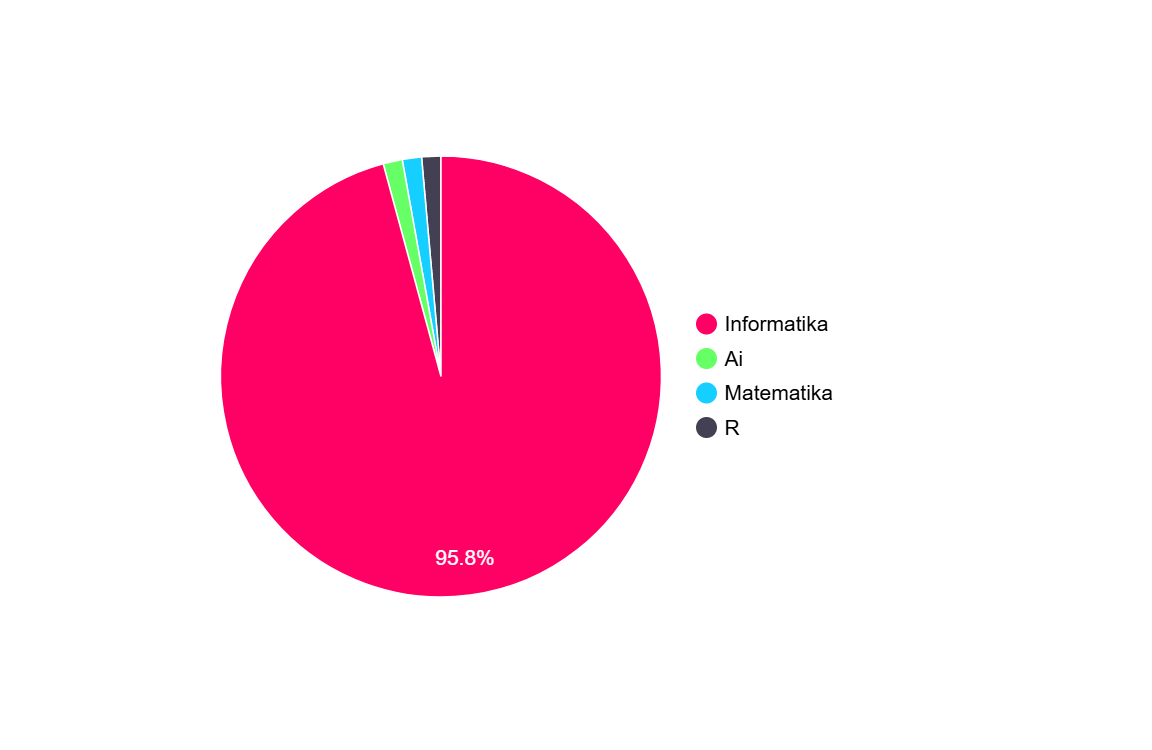
\includegraphics[width=0.7\linewidth]{Slike/PieChartSmerovi.png}
    \caption{Raspodela ispitanika po studijskim programima Matematičkog fakulteta}
    \label{fig:raspodela_smerovi}
\end{figure}


Najveći procenat ispitanika \textbf{(31.9\%)} pohađa master studije, praćeno studentima treće \textbf{(19.4\%)}, druge \textbf{(13.9\%)} i četvrte \textbf{(11.1\%)} godine studija. Preostali ispitanici se deklarišu kao studenti prve godine \textbf{(8.3\%)}, studenti produženih osnovnih studija \textbf{(11.1\%)} i studenti koji su studije završili \textbf{(4.2\%)}. Prikaz raspodele ispitanika po godinama prikazan je na slici \ref{fig:raspodela_godine}.

\begin{figure}[H]
    \centering
    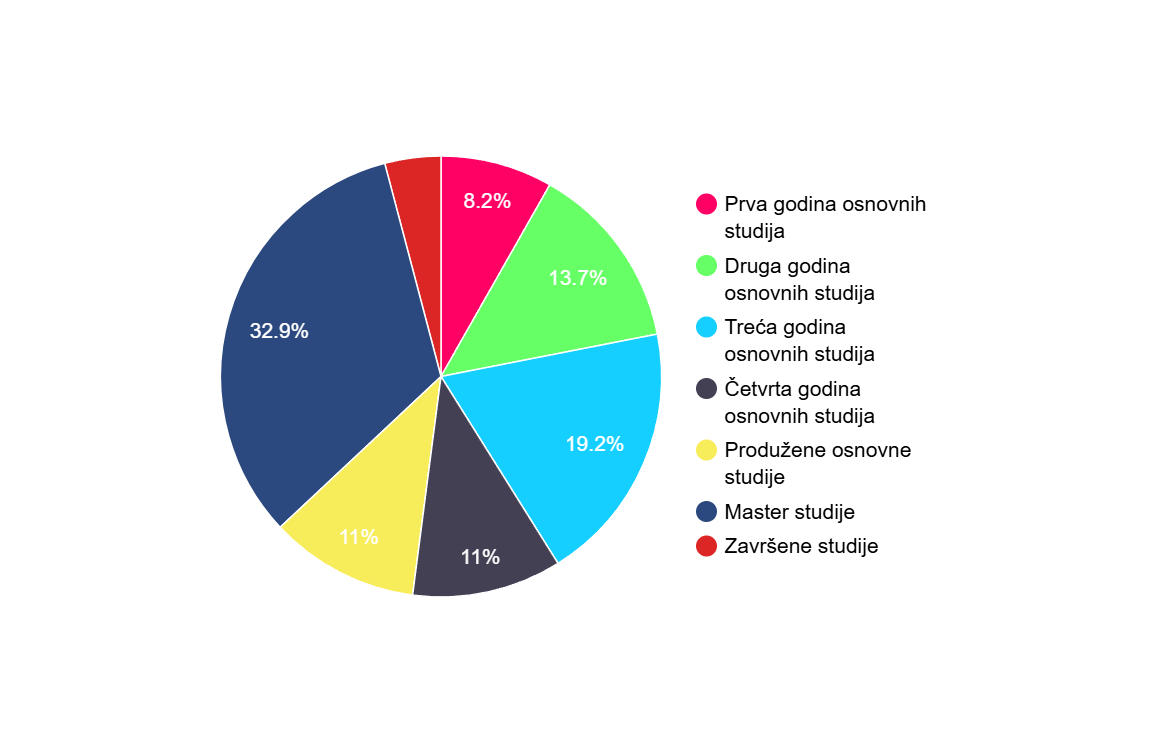
\includegraphics[width=0.7\linewidth]{Slike/PieChartGodinaStudiranja.png}
    \caption{Podela ispitanika po trenutnoj godini studija}
    \label{fig:raspodela_godine}
\end{figure}


Na pitanje o proseku tokom studija, \textbf{50\%} ispitanika odgovorilo je da im prosek iznosi između 7 i 7.99, \textbf{22.1\%} ima prosek između 8 i 8.99, dok čak \textbf{16.2\%} ispitanika ima prosek u opsegu od 9 do 10. Samo \textbf{4.4\%} ispitanika ima prosek između 6 i 7, dok preostalih \textbf{7.4\%} nije želelo da se izjasni. Raspodela proseka može se videti na slici \ref{fig:raspodela_prosek}. Takođe, procenat ispitanika ženskog pola iznosi \textbf{(41.7\%)} dok procenat ispitanika muškog pola iznosi \textbf{(56.9\%)}. Ostalih \textbf{(1.4\%)} ispitanika se nije izjašnjavalo o polu.

\begin{figure}[H]
    \centering
    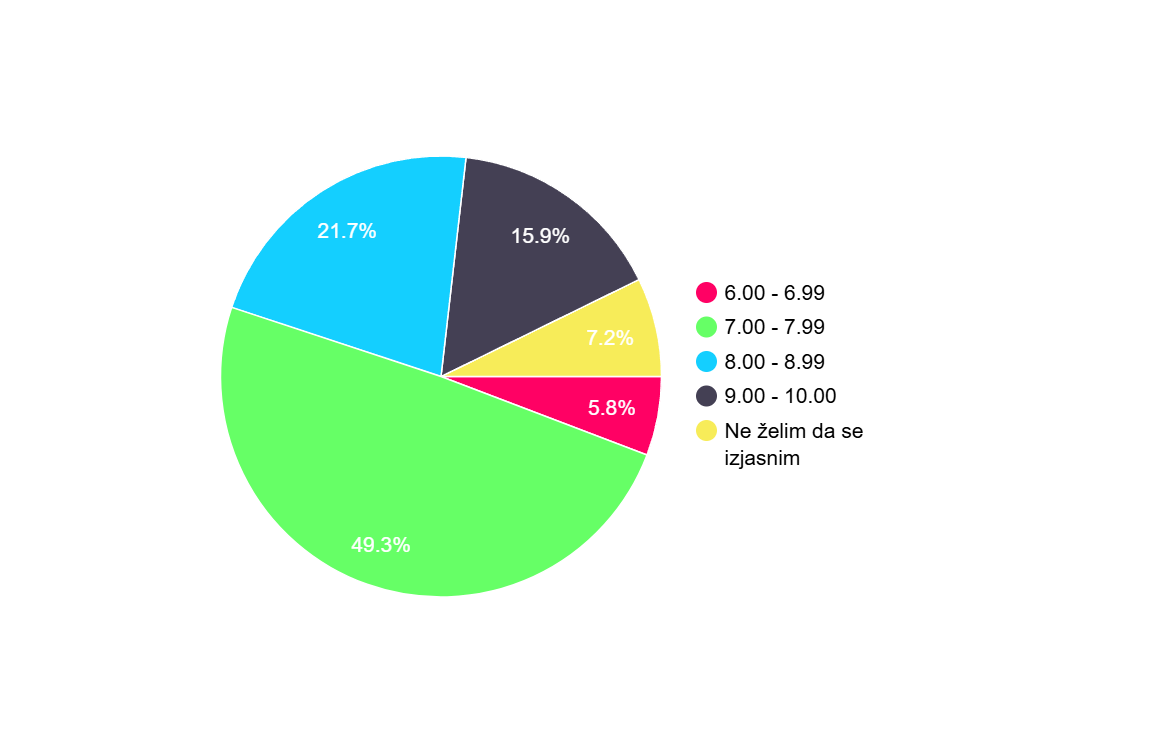
\includegraphics[width=0.7\linewidth]{Slike/PieChartProsek.png}
    \caption{Podela ispitanika po proseku}
    \label{fig:raspodela_prosek}
\end{figure}

\section{Stavovi studenata}
\label{sec:stavovi}


U ovom odeljku ćemo se pozabaviti stavovima ispitanih studenata koji su u vezi sa postavljenim kriterijumima idealnog studiranja. Iako smo već ranije postavili te kriterijume, smatramo da je neophodno da ispitamo koliko su studentima ti kriterijumi važni da bi studije bile idealne. Ukoliko te kriterijume ne smatraju važnim, postavljati pitanja o njihovim iskustvima, koja su u vezi sa datim kriterijumima, postaje besmisleno.


\subsection{Zadovoljstvo kursevima}
\label{subsec:zadovoljstvo_stavovi}

Zadovoljstvo studenata kursevima koje pohadjaju je značajan činilac koji doprinosi poboljšanju kvaliteta tih kurseva, kao i celokupnom kvalitetu studija \cite{satisfaction}. Bitno je baviti se opštim zadovoljstvom studenata kako bi se proverilo da li studije ispunjavaju svoju namenu. Naime, ta namena je da pripreme studente za izazove koji im slede u daljim karijerama \cite{education}. Ovde se takođe nameću i kriterijumi pripreme studenata da mogu samostalo da se usavršavaju nakon završenih studija, kao i koliko predmeti prate potrebe tržišta, ali o tome kasnije.

Anketom je ispitano zadovoljstvo studenata obaveznim i izbornim predmetima. Na pitanje koliko misle da je bitno da student bude zadovoljan obaveznim kursevima, \textbf{54.3\%} ispitanika je dalo najvišu ocenu, ocenu 4 je dalo \textbf{28.6\%} ispitanih studenata. Znači da je čak \textbf{83\%} ispitanika reklo da se slaže sa tvrdnjom da je zadovoljstvo studenata važno. Prosečna ocena je 4.32, medijana je 5, dok je varijansa 0.76.

Za izborne predmete je situacija slična, s tim što je veći broj studenata najvišom ocenom ocenilo važnost zadovoljstva izbornim predmetima, čak \textbf{70\%}, dok je ocenu 4 dalo \textbf{21.4\%} ispitanika. Što znači da je čak \textbf{91.4\%} ispitanih studenata reklo da je njihovo zadovoljstvo izbornim predmetima važno kako bi se studije smatrale idealnim. Prosečna ocena je 4.58, medijana je 5, dok je varijansa 0.55. Iz prethodnih rezultata zaključujemo da je studentima vrlo važno da budu zadovoljni kursevima koje pohađaju kako bi studije bile idealne.


\subsection{Osnova za samostalno usavršavanje}
\label{subsec:usavršavanje_stavovi}
Kao što je malopre pomenuto, primarni cilj studija je da studenti postanu dovoljno vešti da mogu savladati sve izazove na koje mogu naići u svojoj predstojećoj karijeri. Ova tvrdnja je važna i nama deluje da se nedovoljno o njoj diskutuje. Problemi koji mogu nastati usled nedostatka posla su brojni \cite{job_lacking}. Osim toga, konkurencija za posao raste dok broj poslova opada \cite{job_competiton}. Stoga je bitno da studenti imaju neki vid garancije da neće strahovati da li će uspeti da pronađu posao posle studija.
Teško je predvideti kako će se potrebe tržišta menjati \cite{job_prediction}. Takođe, nije ni izvodljivo da se student nauči svemu \cite{learn_everything}. Zato je bitno usredsrediti se na znanja koja pružaju dobru osnovu. Kako bi studenti nakon završetka studija, shodno potrebama mogli nadalje saim usavršavati svoja znanja sa što manje poteškoća.

Motivisani ovim tvrdnjama, u anketi je postavljeno pitanje da li smatraju da je za idealne studije bitno da se stiče dobra osnova koja omogućava samostalno usavršavanje kasnije. Najčešći odgovor je bio da se u potpunosti slažu (ocena 5), čak \textbf{66.7\%} odgovora, ocenu 4 ja dalo \textbf{25\%}, dok je srednju (ocenu 3) dalo samo \textbf{5.6\%} studenata. Prosečna ocena iznosi 4.54, medijana je 5, dok je varijansa 0.61. Odgovori su skoro jednoglasni po stavu da je važno da idealne studije treba da spreme studente za svoje dalje poduhvate. 

\subsection{Kursevi koji prate tržište}
\label{subsec:tržište_stavovi}
Utvrdili smo da je važno da studenti steknu imaju dobru osnovu. Pored toga, važno je i da po završetku studija budu spremni za rad, bez potrebe za dodatnim usavršavanjem odmah na početku karijere.
S tim u vezi, smatramo da je bitno razmotriti da li su obrađivane teme na kursevima u skladu sa potrebama tržišta. Ukoliko nisu, mišljenja smo da bi to ograničilo studije samo za potrebe bavljenja naučnim radovima.

Pitanje koje smo postavili u anketi, kako bismo uvideli značaj ovog uviđanja, je: da li smatrate da je za idealne studije važno da su predmeti povezani sa potrebama tržišta? Najčešća ocena je bila 4 ( \textbf{43.7\%}), najveću ocenu (ocenu 5) je dalo \textbf{35.2\%}, niske ocene (1 i 2) je dalo ukupno \textbf{10\%} ispitanih studenata. Prosečna ocena je 4, medijana je 4, dok je varijansa 1.03. Odavde se može zaključiti da je pomenuti kriterijum smatran za važnim među ispitanicima.


\subsection{Organizacija fakulteta i kurseva}
\label{subsec:organizacija_stavovi}

U okviru već pomenute ankete, postavljena su pitanja o tome da li oni smatraju da je organizacija fakulteta bitna za idealne studije. Preko \textbf{70\%} ispitanika se izjasnilo da se u potpunosti slažu (ocena 5) sa stavom da je organizacija bitna za idealne studije.
\begin{figure}[h!]
\begin{center}
    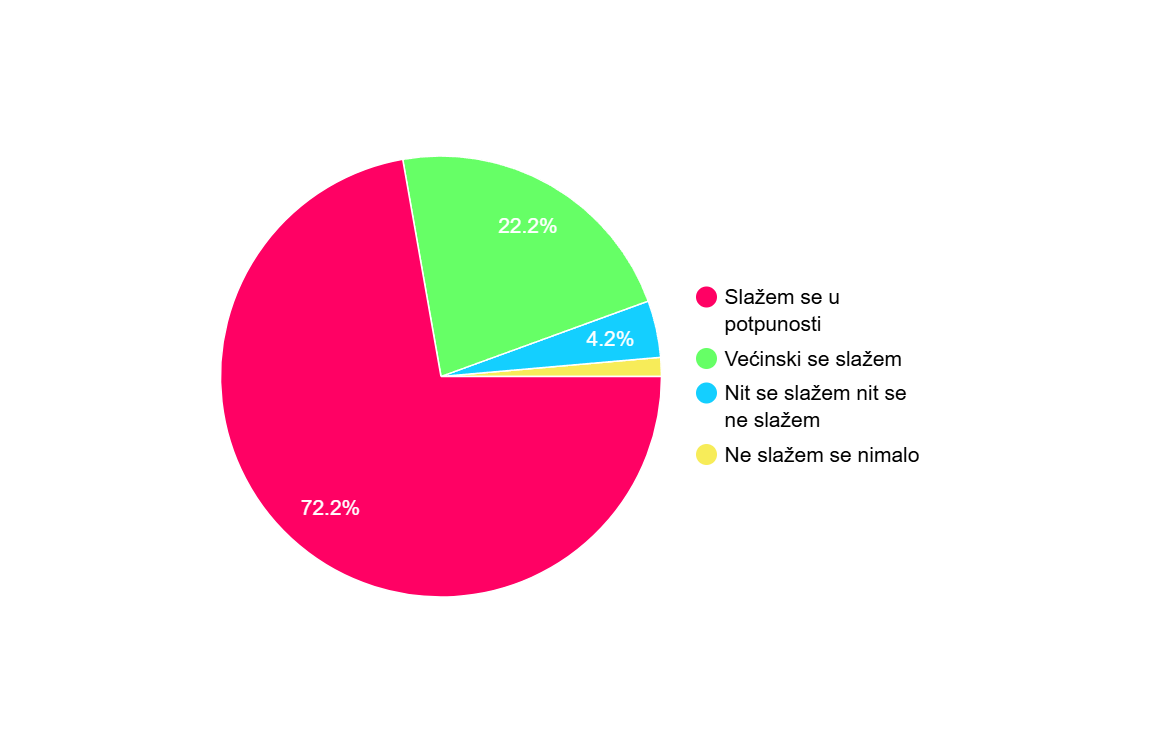
\includegraphics[width=0.7\linewidth]{Slike/PieChartOrganizacijaFakulteta.png}
    \caption{Stavovi studenata o tome koliko je organizacija fakulteta bitna za kvalitet studija}
    \label{fig:organizacija}
\end{center}
\end{figure}

Takođe, većina studenata smatra da je za kvalitet studija bitno da imaju uticaj na to kako se kursevi polažu. Opcija da studenti biraju da li će imati predispitne obaveze ili projekte im pomaže da savlaju gradivo, što dalje utiče njihovo poimanje da li su studije idealne.
\begin{figure}[h!]
\begin{center}
    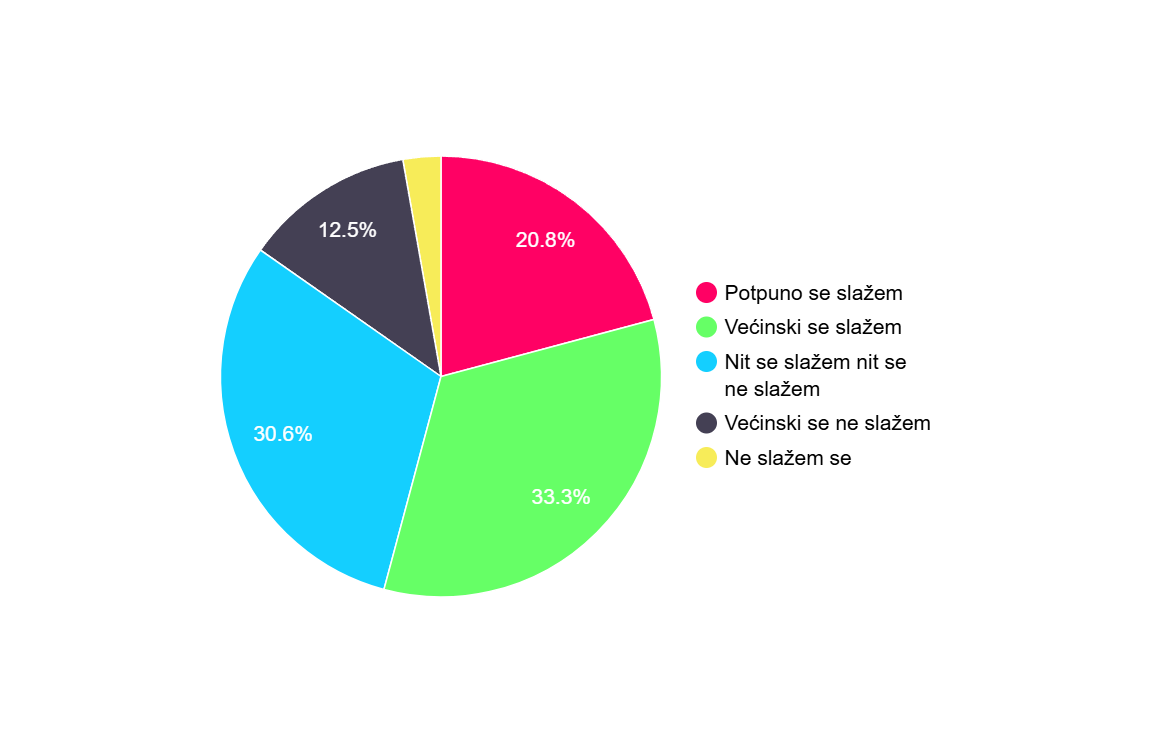
\includegraphics[width=0.7\linewidth]{Slike/PieChartNacinPolaganja.png}
    \caption{Stavovi studenata o tome koliko je bitno da imaju uticaj na to kako se ispiti polažu}
    \label{fig:uticaj}
\end{center}
\end{figure}


\begin{figure}[h!]
\begin{center}
    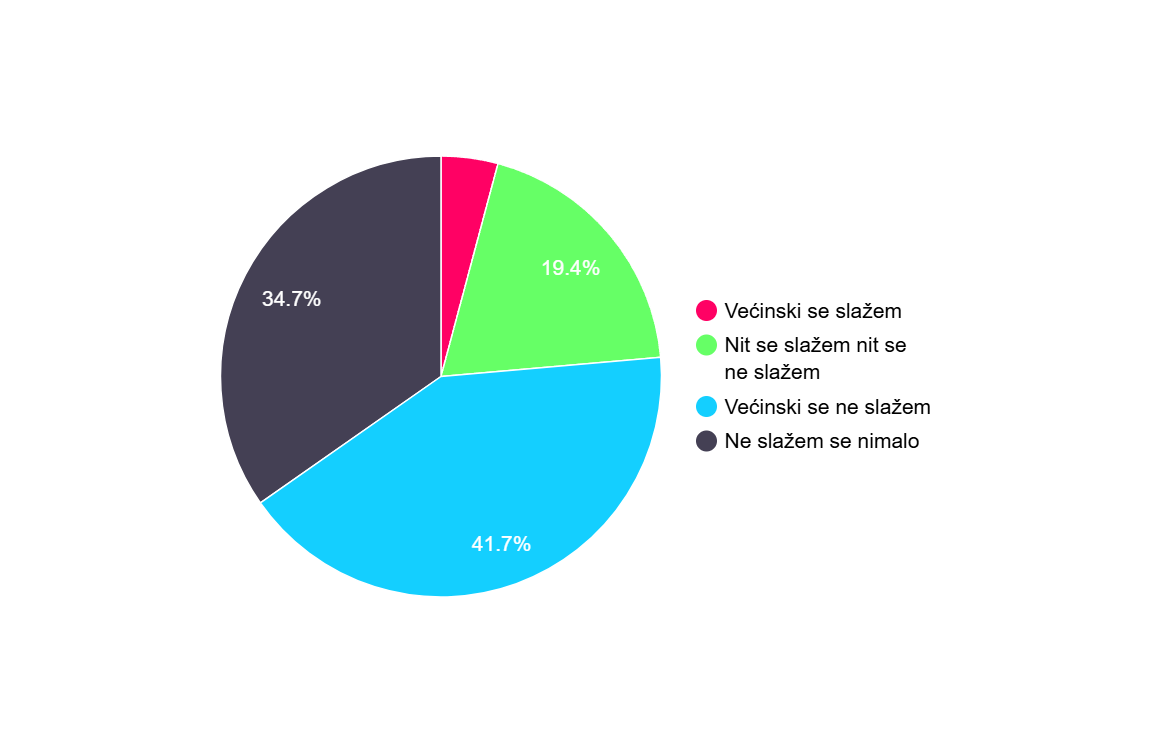
\includegraphics[width=0.7\linewidth]{Slike/PieChartOrganizacijaMatfa.png}
    \caption{Ocene organizacije na Matematičkom fakultetu}
    \label{fig:organizacija_matf}
\end{center}
\end{figure}

Ranije smo pomenuli usaglašenost kurseva sa industrijom \ref{subsec:tržište_stavovi}, kao i organizaciju fakulteta. Valjalo bi sada pogledati kako studenti gledaju na mogućnost dobijanja praksi za vreme studija, koje su organizovane od strane fakulteta. Čak \textbf{90\%} ispitanih studenata je reklo da smatraju da je važno da fakultet ima obavezu obezbeđivanja prilika za praksom. Odnosno, da im bar omogući saradnju sa kompanijama za vreme studija.

\subsection{Povratne informacije o napretku studenata}
\label{subsec:povrane_informacije}

Samopouzdanje studenata je podatak na osnovu kog se može predvideti njihov napredak\cite{correlation}.
Profesori i mentori imaju uticaj na samopouzdanje svojih učenika. Stoga imaju i odgovornost da samopouzdanje raste, a ne da opada.

Ukoliko se desi da je samopouzdanje nisko onda će to negativno uticati na napredak studenta \cite{confidence}. Sa drgue strane, povratne informacije o napretku pozitivno utiču na samopouzdanje studenata. Studenti koji su sigurni u sebe i svoje znanje će bolje predstaviti sebe prilikom nalaženja posla. Takođe će i nakon studija za uzvrat oceniti svoj fakultet bolje. 

Većina ispitanika smatra da je za idealne studije neophodno da u toku studija često dobijaju povratne informacije kako bi se osećali sigurnije u svoje znanje. 
\begin{figure}[h!]
\begin{center}
    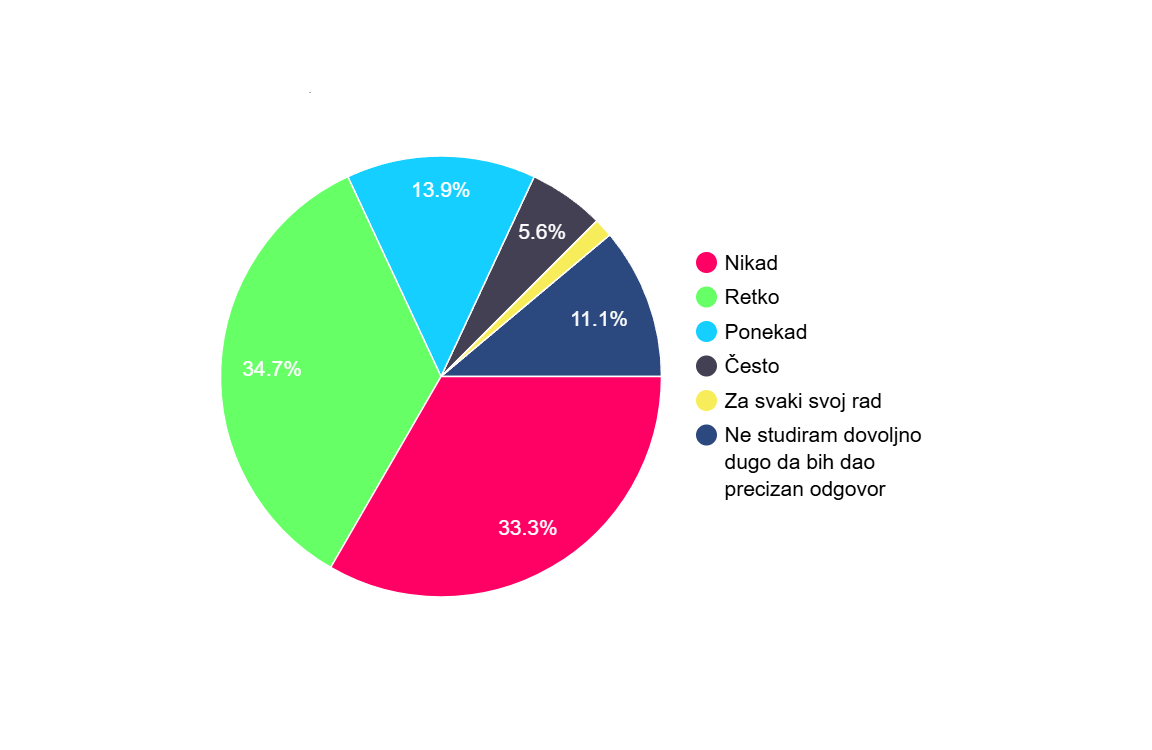
\includegraphics[width=0.7\linewidth]{Slike/PieChartPovratneInformacije.png}
    \caption{Stavovi o važnosti povratnih informacije u toku studija}
    \label{fig:povratne_informacije}
\end{center}
\end{figure}

\section{Iskustva studenata na Matematičkom fakultetu}
\label{sec:iskustva}

Dosad smo se bavili kriterijumima i studentskoj saglasnosti o njihovoj važnosti. Sada ćemo obrađivati rezultate o iskustvima studenata o tim istim kriterijumima. Na osnovu tih rezultata ćemo istaći šta mi mislimo da te ocene govore o zastupljenosti kriterijuma u praksi.  

\subsection{Zadovoljstvo kursevima}
\label{subsec:zadovoljstvo_iskustva}
Ispitani studenti su bili jasni kod svojih stavova po pitanju važnosti zadovoljstva obaveznih i izbornih kurseva da bi studije bile idealne \ref{subsec:zadovoljstvo_iskustva}. Sada ćemo videti da li su ti isti ispitanici zadovoljni kursevima koje su pohadjali za vreme studiranja.

Na pitanje koliko su zadovoljni obaveznim predmetima, najviše njih je dalo ocenu 4 (uglavnom zadovoljni), preciznije \textbf{40.3\%}, dok je najvišu ocenu (5, u potpunosti zadovoljni) dalo samo \textbf{13.9\%}, srednju ocenu je dalo 30.6\%, dok je nisku ocenu (ocenu 2) dalo 13.9\% ispitanika. Prosečna ocena iznosi 3.52, medijana je 4, dok je varijansa 0.89.

Kod odgovora u vezi sa izbornim predmetima se javlja slična situacija, 36.1\% je dalo ocenu 4, samo 5.6\% je dalo ocenu 5, srednju ocenu (ocenu 3) je dalo 33.3\% , dok je 25\% dalo niske ocene, po 12.5\% ispitanih studenata ocenu 2, odnosno 1. Prosek ocena iznosi 3.09, medijana je 3, dok je varijansa 1.19. 

Kod oba kriterijuma su studenti ocenili svoje zadovoljstvo kursevima kao prosečno. Naime, po mišljenjima autora, ocena je niža nego što bi trebalo da bude ako je cilj ostvariti idealne studije.

\subsection{Osnova za samostalno usavršavanje}
\label{subsec:usavršavanje_iskustva}
Većina studenata je već okarakterisalo kriterijum spremanja za dalje usavršavanje važnim da bi studije bile idealne \ref{subsec:usavršavanje_stavovi}. Sada treba videti koliko njih je zapravo reklo da je to trend i na Matematičkom fakultetu.
Odgovori su sledeći: \textbf{55.7\%} se uglavnom slaže (ocena 4), \textbf{22.9\%} se slaže u potpunosti, i 11.4\% ispitanika je dalo srednju ocenu (ostali ispitani studenti su rekli da su još uvek na početku studija, te nisu dovoljno studirali kako bi dali precizan odgovor). Prosečna ocena ovih odgovora (računaju se samo oni na skali 1-5) je  4.12, medijana je 4, dok je varijansa 0.6. Gledajući ocenu, vidimo se studenti uglavnom slažu po ovom pitanju, stoga se može tvrditi da smatraju da će biti dobro pripremljeni da se nadalje samostalno usavršavaju shodno izazovima i potrebama.


\subsection{Kursevi koji prate tržište}
\label{subsec:tržište_iskustva}

Već je (anketom) ranije obrađeno da je važno da kursevi prate tržište \ref{subsec:tržište_stavovi}, kad je reč o idealnom studiranju. Stoga, bi sada trebalo ispitati da li se po mišljenju ispitanika smatra da je on zastupljen i u praksi. Gledajući rezultate ankete, najčešće je data srednja ocena (ocena 3) \textbf{50\%}, visoka ocena (ocena 4)\textbf{27.8\%}, najviša ocena samo \textbf{4.2\%} među svim odgovorima, dok je ostalo niska ocena. Prosečna ocena je 3.11, medijana 3, varijansa 0.82. Ako bismo uzeli date rezultate u obzir, reklo bi se da kursevi donekle prate potrebe tržišta, ali da su još uvek nezavisni u odnosu na tržište. Što odstupa od stava da treba da budu u vezi sa tržištem, ako je cilj da se studije smatraju idealnim.

\subsection{Organizacija fakulteta i kurseva}
\label{subsec:organizacija_iskustva}

Kada smo tražili od ispitanika da ocene organizaciju na Matematičkom fakultetu, većina studenata nije bilo zadovoljno. Naime, \textbf{76\%} ispitanika je dalo ocenu 1 ili ocenu 2. Niko od ispitanika nije dao ocenu 5. Glavni razlog za ovakve odgovore je bio manjak rokova za polaganje ispita, blisko praćen činjenicom da su teorijski i praktični deo ispita najčešće u razdvojenim terminima, ali jako zavisni jedno od drugog.

Ovde ćemo takođe napomenuti i studenstke prakse. Naime, samo \textbf{12.7\%} ispitanika je imalo prilike za studenstkim praksama, od čega je \textbf{72.7\%} došlo samostalno do te prakse. Ovo nam govori da fakultet nema nikakvih veza sa omogućavanjem prilika studentima za praktična usavršavanja. Hteli bismo samo i da napomenemo da se protiv ovog stava može argumentovati time da je fakultet odradio svoj deo posla omogućivši dovoljno znanja studentima da budu samostalno primljeni na te prakse. Ali uzevši u obzir prethodnu priču o stanjima na tržištu \ref{subsec:tržište_stavovi}, svaki vid prednosti je značajan.

\subsection{Povratne informacije o napretku studenata}
\label{subsec:napredak_iskustva}
Na Matematičkom fakultetu studenti se većinski slažu da skoro nikada nisu dobijali povratne informacije o svom napretku tokom studija. Čak \textbf{67.6\%} studenata je reklo da su jako retko ili da nikada nisu dobijali ovu vrstu povratne informacije, što je negativno uticalo na njihov napredak. Ova činjenica ima uticaj na samopouzdanje studenata, pa su iz tog razloga ove vrste potvrda neophodne kako bi studije bile idealne. 
\begin{figure}[h!]
\begin{center}
    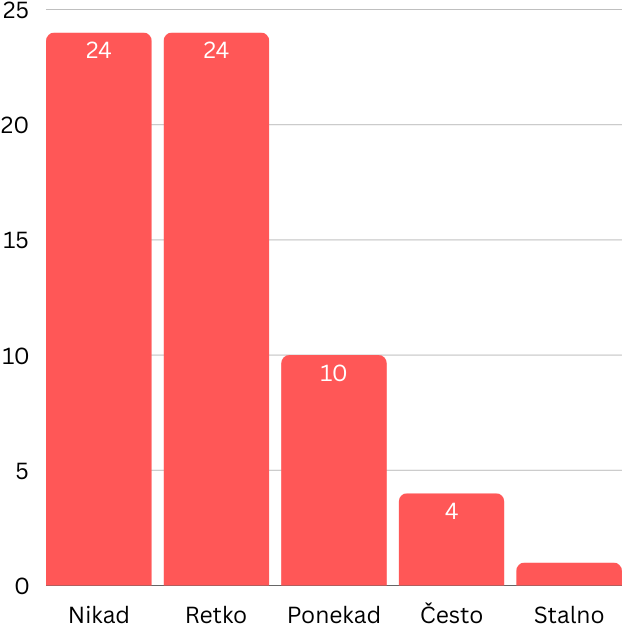
\includegraphics[scale = 0.3]{PovratneInformacijeMatf.png}
    \caption{Učestalost povratnih informacija o napretku na Matematičkom fakultetu}
    \label{fig:povratne_informacije_matf}
\end{center}
\end{figure}

Većina studenata Matematičkog fakulteta (njih 32) je donekle siguran u svoje znanje. Potpuno sigurnih studenata (njih 9) ima isto koliko i onih koji nisu uopšte sigurni (njih 1) ili su većinski nesigurni (njih 8).
\begin{figure}[h!]
\begin{center}
    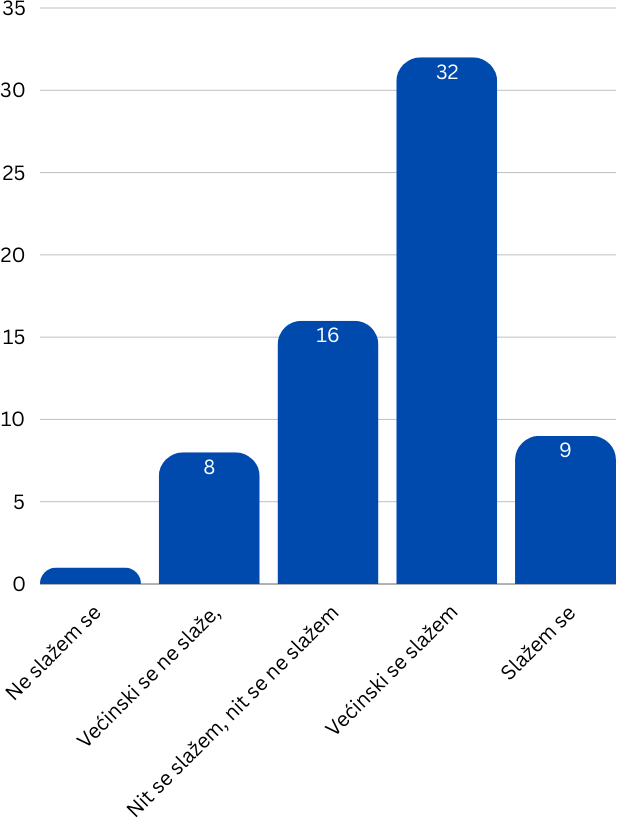
\includegraphics[scale = 0.3]{SamouverenostStudenataMatf.png}
    \caption{Koliko su studenti Matematičkog fakulteta samouvereni u svoje znanje}
    \label{fig:samouverenost_matf}
\end{center}
\end{figure}


\section{Zaključak}
\label{sec:zakljucak}

Na osnovu obrađenih rezultata mogli smo videti da su među bitnijim kriterijumima navedeni kursevi, njihova zastupljenost na tržištu kao i koliko dobru osnovu obezbeđuju studentima. Pored toga videli smo da organizacija na fakultetu, kao i odnos prema studentima imaju svoj doprinos kako bi se studije učinile idealnim. 

Rezultati pokazuju da ostvarivanje ovih kriterijuma u praksi (bar na Matematičkom fakultetu)odstupa od najvišeg standarda. Matematički fakultet kao visokoškolska ustanova imanpotencijala, ali iz iskustva studenata deluje kao da se ne radi dovoljno na tome da se studije približe statusu idealnih. 

Iako možda još uvek nije idealan, daleko je od lošeg. Deluje kao da dosta stvari treba menjati, međutim trebalo bi se osvrnuti na stvari koje su zaista na zadovoljavajuće visokom nivou i podjednako raditi na tome da se te osobine očuvaju.  


\addcontentsline{toc}{section}{Literatura}
\appendix
\bibliography{seminarski} 
\bibliographystyle{plain}

\appendix
\section{Dodatak}

Dodatno, pitali smo ispitanike da nam daju neke predloge kako oni misle da bi se studije na Matematičkom fakultetu mogle unaprediti. Dobili smo dvadeset i četiri različita korisna odgovora u kojima se nalazi devet različitih ideja, a najčešće su prikazane u tabeli ispod, uparene sa brojem pojavljivanja.\\

\begin{table}[h!]
\begin{center}

\begin{tabular}{|c|c|} \hline
Ideja& Broj ponavljanja\\ \hline

Povećanje količine opcionih predispitnih obaveza & 5\\ \hline
Povećanje broja rokova & 4\\ \hline
Veća dostupnost potrebne literature na internetu & 4\\ \hline
Omogućiti odvojeno polaganje teorije i praktičnog ispita & 3\\ \hline
\end{tabular}
\label{tab:tabela1}
\caption{Ideje studenata kako se studije na Matematičkom fakultetu mogu unaprediti}
\end{center}
\end{table}

Većina studenata ima mišljenje da bi bar jedna od ove četiri promene drastično uticala na kvalitet studija na Matematičkom fakultetu.

\end{document}